\documentclass[10pt,letterpaper]{article}
%\pdfoutput=1 

%\usepackage[utf8]{inputenc}

\def\baselinestretch{1.06} 
\usepackage{geometry}
\geometry{letterpaper,tmargin=2.0cm,bmargin=2.0cm,lmargin=3.0cm,rmargin=3.0cm}
\usepackage[english]{babel}


\setlength{\parskip}{0.1in}
\hyphenpenalty=1000

%\usepackage[babel]{csquotes}
\usepackage{amsmath,amsfonts,amssymb,amsthm}
%\usepackage{mathtools}
\usepackage{mathrsfs}
%\usepackage{bm}
\def\zb{\bar{z}}
\def\sO{\mathrm{O}}
\def\msf{\mathsf}
\def\eps{\epsilon}
\def\ga{\gamma}
\def\bh{\mathbf{h}}
\def\a{\alpha}
\def\b{\beta}
\usepackage{graphicx}
%\usepackage{comment}
%\usepackage{booktabs}
%\usepackage{array}
\usepackage{dsfont}
\def\mrm{\mathrm}
\def\unit{\mathds{1}} % needs dsfont package
%\usepackage{showkeys}
\def\mbf{\mathbf}
\newcommand{\NO}[1]{{:\!#1\!:}}
\def\Oo{\mathcal{O}}
\def\Red{\color [rgb]{0.9,0.1,0.1}}
\def\Blue{\color [rgb]{0.0,0.2,0.7}}

\newcommand{\vx}{\vec{x}}


\def\tr{\mrm{Tr}}
\def\bM {\mathbb{M}} 
\def\bR {\mathbb{R}} 
\def\vareps{\varepsilon}
\def\DD{\Delta}
\def\dd{\delta}
\def\aa{\alpha}
\def\bb{\beta}
\def\pd{\partial}
\def\mfr{\mathfrak}
\newcommand{\CG}{{$SO(d+1,1)$}}
\newcommand\be{\begin{equation}}
\newcommand\ee{\end{equation}} 
\newcommand\beq{\begin{equation}}
\newcommand\eeq{\end{equation}} 
\newcommand\D{\Delta}
\newcommand\g{\gamma} 
\newcommand\G{\Gamma} 
\newcommand\e{\epsilon} 
\newcommand\la{\lambda}
\newcommand\Op{\mathcal{O}}
\newcommand\Ocal{\mathcal{O}}
\newcommand\Ncal{\mathcal{N}}
\renewcommand{\cal}{\mathcal}
\renewcommand{\a}{\alpha} 
\renewcommand{\b}{\beta}
\renewcommand{\d}{\delta} 

\newcommand{\ceil}[1]{\left \lceil #1 \right \rceil }
\newcommand{\floor}[1]{\left \lfloor #1 \right \rfloor }
\newcommand{\braket}[3]{\langle #1|#2|#3 \rangle}
\newcommand{\brakket}[2]{\langle #1|#2\rangle}
\newcommand{\ket}[1]{|#1\rangle}
\newcommand{\bra}[1]{\langle #1|}
\newcommand{\expec}[1]{\langle #1 \rangle}
\newcommand{\no}[1]{:\! #1 \!:}

\renewcommand{\bf}{\textbf}
\renewcommand{\rm}{\textrm}
\renewcommand{\it}{\textit}

\def\ldef{\mathrel{\mathop:}=}
\def\rdef{=\mathrel{\mathop:}}

\newcommand{\reef}[1]{(\ref{#1})}
\usepackage{xcolor}
\definecolor{darkblue}{rgb}{0.1,0.1,.7}
\usepackage[colorlinks, linkcolor=darkblue, citecolor=darkblue, urlcolor=darkblue, linktocpage]{hyperref} 
\newcommand{\limu}[1]{\mathrel{\mathop{\sim}\limits_{\scriptstyle{#1}}}}
\def\nn{\nonumber} 
\def\bsub{\begin{subequations}}
\def\esub{\end{subequations}}
\def\xh{\hat{x}}
\def\half{\frac{1}{2}}
\def\mbb{\mathbb}
\def\mca{\mathcal}
\def\wh{\widehat}
\def\lra{\leftrightarrow}
\def\msc{\mathscr}
\def\qaq{\quad\text{and}\quad}
\newcommand{\ud}[2]{^{#1}_{\phantom{#1}#2}}
\newcommand{\du}[2]{_{#1}^{\phantom{#1}#2}}
\def\th{\tfrac{1}{2}}


\begin{document}


\title{Susceptibility of the Ising model}
\author{Matthijs Hogervorst}
\date\today
\maketitle

Consider the Ising model on a finite lattice of size $V = L^d$. There
are $2^V$ configurations $\{\sigma_x\}_x$, $\sigma_x = \pm 1$. The
Hamiltonian is
\beq
H = - \sum_{\expec{x,y}} \sigma_x \sigma_y,
\quad
Z = \sum_{\sigma} e^{-\beta H}.
\eeq
The susceptibility is
\beq
\chi \ldef \expec{\mca{X}} = \frac{1}{Z} \sum_\sigma \mca{X} e^{-\beta H},
\quad
\mca{X} \ldef \frac{1}{V^2} \sum_{x,y} \sigma_x \sigma_y.
\eeq
Note that
\beq
\mca{X} = \left(\frac{1}{V} \sum_x \sigma_x\right)^2 \geq 0
\eeq
meaning that $\mca{X} \geq 0$ for \emph{every} configuration
$\{\sigma_x\}_x$. Moreover clearly $\mca{X} \leq 1$. We can measure
$\chi$ directly for small $V$, by summing over all $2^V$
configurations. The results are shown in Fig.~\ref{fig:susc}.
\begin{figure}[htbp]
  \begin{center}
    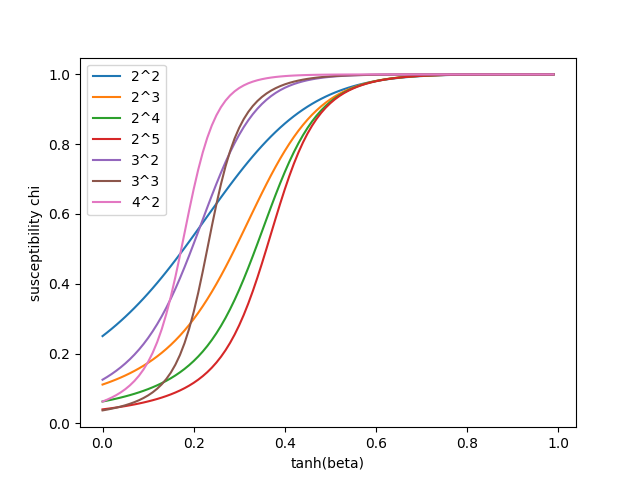
\includegraphics[scale=0.5]{suscepPlot.png}
    \caption{\label{fig:susc}Susceptibility for a range of different lattices,
      scanning over $\tanh(\beta)$.}
  \end{center}
\end{figure}

Moreover notice that for any observable $\Oo$
\beq
\frac{\pd \expec{\Oo}}{\pd \beta} = \expec{\Oo} E -  \expec{\Oo H}
\quad
\Rightarrow
\quad
\frac{\pd\chi}{\pd\beta} = \chi \cdot E - \expec{\mca{X} H}.
\eeq
Using this, we can compute $\pd_\beta \chi$ directly too; see Fig.~\ref{fig:ds}.
\begin{figure}[htb]
  \begin{center}
    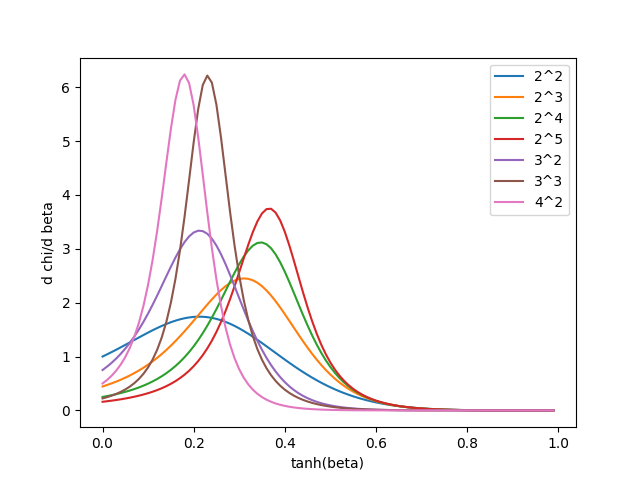
\includegraphics[scale=.5]{der_suscepPlot.png}
    \caption{\label{fig:ds}Derivative of the
      susceptibility (right) for a range of different lattices,
      scanning over $\tanh(\beta)$.}
  \end{center}
\end{figure}
Finally we can plot the energy, see Fig.~\ref{fig:en}.
\begin{figure}[htb]
  \begin{center}
    \hspace{0mm}
    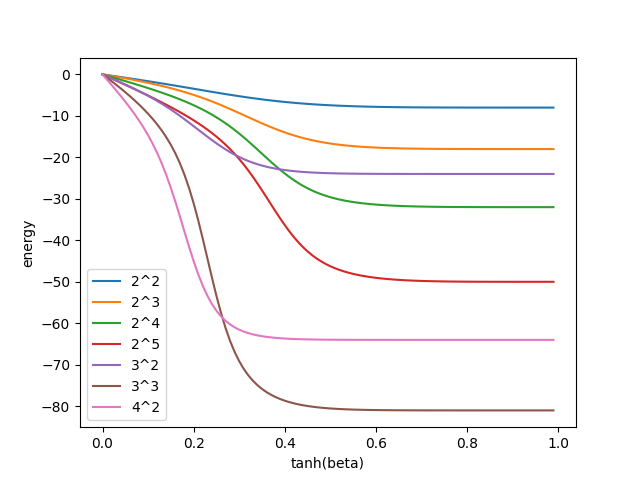
\includegraphics[scale=.5]{energyPlot.png}
    \caption{\label{fig:en}Energy $\expec{H}$ for a range of different lattices,
      scanning over $\tanh(\beta)$.}
  \end{center}
\end{figure}

As for analytics, we can show that
\beq
\chi \, \limu{\beta \to 0} \,  \frac{1}{V} + \frac{2d}{V}\, \tanh(\beta) + \ldots
\qaq
\chi \limu{\beta \to \infty} 1.
\eeq
For the energy we have
\beq
E \limu{\beta \to 0} 0 \qaq
E \limu{\beta \to \infty} -dV.
\eeq
This seems to agree with the data.

   
\end{document}
